%*****************************************
\chapter{Grundlagen}\label{ch:grundlagen}
%*****************************************
In den folgenden Abschnitten sollen nun Grundlagen betrachtet werden, welche bei der Umsetzung des \ac{IDS} nötig sind.
    Essentiell dabei sind zum einen die Definition von Anomalien und der Anomaliedetektion (siehe Kapitel~\ref{sec:Anomalieerkennung})
    und eine allgemeine Einführung in den Bereich der \ac{IDS} (siehe Kapitel~\ref{sec:IDS}).
    Dabei wird auf den im praktischen Teil verwendeten Ansatz der \textit{Host-Based Intrusion Detection Systems} (HIDS) genauer eingegangen.
    Nachdem so eine allgemeine Herangehensweise an die Erkennung von Angriffen dargelegt wurde, 
    soll im Anschluss die Grundlagen des verwendeten Algorithmus untersucht werden.
    Dazu gehören rekurrente neuronale Netze (RNN), sowie die Erweiterung der RNNs die \textit{Long Short-Term Memory} neuronalen Netzen (LSTM)\@.

    \section{Intrusion Detection System}\label{sec:IDS}
        Eine \textit{Intrusion} \marginpar{zu dt. Eindringung} ist eine unauthorisierte Aktivität, welche einem System Schaden zufügen kann.
        Eine \textit{Intrusion Detection} Software/Hardware versucht automatisch diese 
        unauthorisierten Aktivitäten zu identifizieren, um dadurch die Sicherheit des Systems gewährleisten zu können.~\cite{IDSreview}
        Um solche unautorisierte Aktivitäten erkennen zu können müssen zunächst Daten erfasst und anschliessend analysiert werden.
        In den folgenden beiden Abschnitten werden diese Schritte genauer untersucht.

        \subsection{Datenanalyse}\label{sec:Datenanalyse}
        Das Erkennen von Angriffen auf Computersystemen mittels \ac{IDS} wird meist, wie auch in~\cite{IDSreview} und~\cite{IDSsurvey}, in drei Kategorien eingeteilt.
            Dazu zählen die signaturbasierten und anomaliebasierten Verfahren auf die im Folgenden eingegangen wird,
            sowie die \textit{Stateful Protocol Analysis} \marginpar{zu dt. Zustandsorientierte Protokoll Analyse}.

            \paragraph{Signaturbasiert} 
                \ac{SIDS} versuchen Muster von bekannten Angriffen 
                in den zu überwachenden Systemen wiederzuerkennen.
                Dies basiert darauf, eine ausgeprägte Datenbank an Signaturen von bekannten Angriffen zu besitzen.
                Verschiedene Methoden vergleichen dann aktuelle Signaturen des Systems mit der Datenbank.
                Es gibt auch hier diverse Methoden wie diese Signaturen erstellt werden. 
                Dazu zählen zum Beispiel das Betrachten von \textit{Host-Logs},
                oder ein wenig ausgefeilter das Erstellen von \textit{State Machines}~\cite{SIDSstate}
                Doch ein wesentlicher Nachteil der signaturbasierten IDS liegt in der Tatsache,
                dass keinerlei neuartigen Angriffe, sowie viele Abwandlungen von Angriffen nicht erkannt werden,
                da diese noch nicht in der Datenbank vorhanden sind.~\cite{IDSsurvey}

            \paragraph{Anomaliebasiert}
                Ziel einer \ac{AIDS} ist es Muster in Daten wiederzuerkennen 
                welche von einem definierten Normalverhalten abweichen~\cite{ANOMALYSURVEY}.
                Die Bedeutung der Anomalieerkennung liegt in der Tatsache begründet,
                dass Anomalien in Daten zu signifikanten und oft kritischen Veränderungen eines System führen können. 
                So kann eine Anomalie in Netzwerkdaten dafür stehen,
                dass ein gekaperter Computer sensitive Daten an ein unautorisiertes Ziel sendet~\cite{ANOMALYEXAMPLE}.
                Anomalien in den Daten können aus verschiedenen Gründen entstehen,
                zum Beispiel durch böswillige Aktivitäten oder aber auch durch Programmfehler.
                Doch alle Anomalien haben gemein,
                dass sie ein Abweichen eines definierten Normalverhalten zeigen und damit interessant für Analysen sind.
                Genau dieser signifikante Unterschied des aktuellen Systemzustand zu dem entworfenen Modell
                (wohldefiniertes Normalverhalten) zu einem Zeitpunkt $t$ wird dann als Anomalie eingestuft.
                %TODO (Details für ML Stat und Knowledge)
                Jede Anomalie gilt dann wiederrum als Intrusion.
                Grundannahme dieser Methode liegt darin, dass Intrusions von dem gelernten Normalverhalten des Systems unterschieden werden können.

                Im ersten Schritt der \ac{AIDS} wird ein Modell des Normalverhaltens erstellt.
                Dabei können ML-basierte, Statistik-basierte oder auch 
                \textit{Knowledge}-basierte \marginpar{zu dt. Wissens-basierte} Algorithmen verwendet werden.
                Weiter kann die anomaliebasierte \textit{Intrusion Detection} in zwei Phasen aufgeteilt werden,
                die \textit{Trainingsphase} sowie die \textit{Testphase}.
                In der ersten Phase wird versucht ein Modell des Programmverhaltens zu ermitteln,
                beziehungsweise zu trainieren.
                In der zweiten soll dieses Modell dann überprüft werden.
                Speziell soll dabei mit noch nicht betrachteten Daten die Generalisierung des Modells getestet werden. 
                Dabei liefert der Algorithmus für jede Eingabe einen Anomaliescore.
                Liegt dieser über einem festgelegten Schwellwert so gilt die Eingabe als 
                \glqq anormal\grqq \ ansonsten als \glqq normal\grqq.
                Die Trainingsphase wird von Chandola et al.~\cite{ANOMALYSURVEY} weiter unterteilt in \textit{Supervised},
                \textit{Semisupervised} sowie \textit{Unsupervised Anomaly Detection}.
                Diese unterscheiden sich hauptsächlich in der Anforderung an den Datensatz. 
                Bei einer \textit{Supervised} Anomalieerkennung werden Trainingsdaten benötigt 
                in welchen Anomalien sowie auch Normalverhalten gelabelt sind.
                Hingegen wird beim \textit{Semisupervised} Verfahren lediglich ein Datensatz benötigt,
                welcher das Normalverhalten kennzeichnet.
                Bei der \textit{Unsupervised Anomaly Detection} werden Daten verwendet welche keine Labels beinhalten.
                Dabei wird davon ausgegangen, dass Normaldaten sehr viel umfangreicher in den Daten vertreten sind als Anomalien,
                da es sonst häufig zu Fehlalarmen kommen kann~\cite{ANOMALYSURVEY2}.
                %TODO kurz erläutern
                Bei der Umsetzung der Anomaliedetektion ergeben sich allerdings einige Schwierigkeiten:
                \begin{itemize}
                    \item \textit{Definition des Normalverhaltens}:
                        Ziel ist es jegliches Verhalten, welches kein anormales beinhaltet, zu erfassen.
                        So muss dafür gesorgt werden,
                        dass das Normalverhalten auch tatsächlich in den Daten widergespiegelt wird. 

                    \item \textit{Dynamik des Normalverhaltens}:
                        Normalverhalten kann sich über die Zeit verändern 
                        und somit vom Algorithmus Gelerntes unbrauchbar machen~\cite{ANOMALYSURVEY}.

                    \item \textit{Datensätze}:
                        Gelabelte Daten zur Erfassung des Normalverhaltens sind oft veraltet oder nicht sehr detailreich. 
                        \marginpar{Mehr dazu in Abschnitt~\ref{sec:Datensatz}}

                    \item \textit{Schwellwert}:
                        Festlegung eines Schwellwertes,
                        welcher die eigentliche Unterscheidung zwischen Normalverhalten und Angriffsverhalten umsetzt.
                \end{itemize}

                %TODO wird bereits im vorigen Kapitel beschrieben
                %Im Allgemeinen besitzen AIDS zwei Phasen, der Trainingsphase und der Testphase.
                %In der Trainingsphase wird ein Modell erstellt welches das Normalverhalten abbilden soll.
                %In der Folgephase muss dann das gelernte Modell mit bisher noch nicht betrachteten Daten überprüft werden.
                %Dabei soll vor allem die Generalisierung des Modells getestet werden. 
                Auch wenn sich die verschiedenen Teilbereiche der \ac{AIDS }stark unterscheiden,
                haben sie einen wesentlichen Vorteil gegenüber den \ac{SIDS}\@.
                Denn ihnen ist es nicht generell verwehrt Zero-Day Angriffe zu erkennen,
                also Angriffe die in dieser Form noch nicht bekannt waren. 
                %Zusätzlich ist es für Angreifende schwer zu ermitteln wie das 
                %AIDS Normalverhalten definiert und diese Definitionsgrenzen auszunutzen um unerkannte Angriffe durchzuführen.
                Jedoch ergibt sich im Vergleich zu den \ac{SIDS} eine andere Problematik.
                Denn die \ac{AIDS} müssen einen Schwellwert festlegen ab welchem ein Vorkommnis als Anomalie erkannt wird.
                Dieser Wert entscheidet über die Ergebnisqualität der \ac{AIDS}
                und sollte daher sorgfältig und am besten automatisch ermittelt werden,
                um anwendungsspezifische Justierungen zu vermeiden. \marginpar{mehr dazu in Kapitel~\ref{sec:Algorithmus}}
                Eine weitere Schwierigkeit bei \ac{AIDS} liegt in der Ermittlung von Daten für das Normalverhalten und die damit verbundene Gefahr,
                dass bei nicht kompletten Erfassen des Normalverhalten viele Fehlalarme enstehen können.
                Daher ist eine entscheidende Frage bei Verwendung von \ac{AIDS}\@: Woher kommen die für das Lernen des Normalverhalten benötigten Daten?
                %Viele verschiedene Ansätze, unter anderem zusammengefasst in~\cite{IDSsurvey}.

        \subsection{Datenerfassung}\label{sec:Datenerfassung}
            Die Datenerhebung wird in verschiedenen Arbeiten in zwei Kategorien unterteilt~\cite{IDSsurvey},~\cite{IDSreview}.
            Zum einen die \ac{HIDS}
            und zum anderen die \ac{NIDS}
            In den folgenden Abschnitten werden diese beiden Ansätze genauer untersucht.

            \paragraph{Network Based Intrusion Detection}
                Überwacht den Netzwerkverkehr über Pakete, NetFlow oder andere Netzwerkdaten.
                Ein großer Vorteil daran ist, dass viele Computer in einem Netzwerk überwacht werden.
                Ziel ist es dabei Angriffe möglichst früh zu erkennen und zu verhindern,
                dass sich die Gefahr weiter ausbreiten kann.
                Doch der erwähnte Vorteil kann schnell zu Schwierigkeiten führen,
                da bei besonders großen Netzen der hohe Datendurchsatz das Erkennen von Angriffen erschwert.~\cite{NIDS}
                Ein weiterer Nachteil bei der Untersuchung von Netzwerkpaketen oder ähnlichem besteht darin,
                dass der Netzwerkverkehr meist verschlüsselt ist
                und somit nicht auf den Inhalt der Pakete eingegangen werden kann.

            \paragraph{Host Based Intrusion Detection}
            Wie der Name bereits impliziert konzentriert sich \ac{HIDS} auf die Untersuchung 
                von Daten welche auf dem Host basieren.
                Es wird versucht das dynamische Verhalten sowie den Zustand des Systems zu überwachen 
                und dies nur mit Informationen die auf dem Host zugänglich sind.
                In der Literatur werden hierfür verschiedene Informationsquellen genutzt.
                Dazu gehören verschiedene Logs, z.B Firewall und Database Logs~\cite{IDSsurvey},
                oder aber auch Daten aus dem Kernel wie z.B. System Calls~\cite{MAGGI}.
                Im Gegensatz zur \ac{NIDS} kann hier auf den Inhalt von jeder Information eingegangen werden,
                da die interne Kommunikation unverschlüsselt stattfindet. 

        Abbildung~\ref{fig:IDSOverview} soll einen Überblick über die in den vorigen Abschnitten gemachte Einstufung geben.
        Dabei gibt die Abbildung die Strukturierung der vorigen Abschnitte wieder,
        in welcher die Datenerfassung in die Host-basierte und Netzwerk-basierte Erfassung unterteilt wird sowie die Datenanalyse
        in die anomaliebasierten und signaturbasierten Verfahren sowie die \textit{Stateful Protocol Analysis} eingeteilt wird.
        Die dicker umrandeten Verfahren werden in dieser Arbeit verwendet.
        Also zur Datenerfassung werden nur Informationen welche auf dem Host zugänglich sind verwendet 
        und die so erhaltenen Daten werden anomaliebasiert untersucht.
        Es stellen sich beim designen von anomaliebasierten \ac{HIDS} zwei Hauptfragen:
        \begin{itemize}
            \item Mit welchen Daten kann das Systemverhalten möglichst präzise dargestellt werden?
                \begin{itemize}
                    \item Logs, System Calls, \dots
                \end{itemize}
            \item Wie wird die eigentliche Anomalie in den Daten erkannt?
        \end{itemize}
        Die erste Frage soll in dem folgenden Abschnitt mit der Betrachtung von System Calls zur Beschreibung des Systemverhaltens angegangen werden.
        Die letztere soll dann speziell in Kapitel~\ref{sec:Algorithmus} beleuchtet werden.

        \begin{figure}[h]
            \centering
            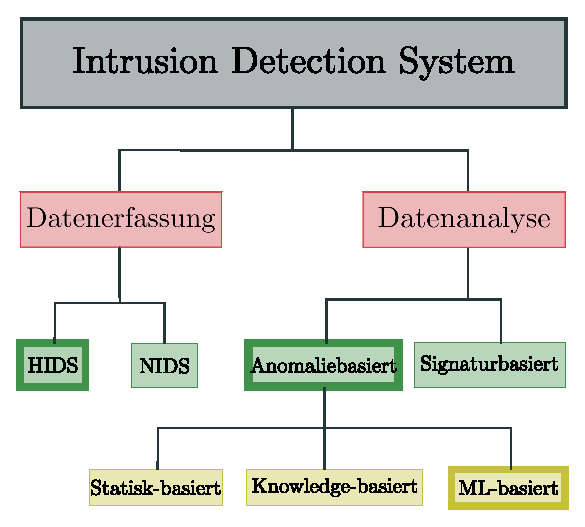
\includegraphics[width=1\textwidth]{images/Illustrationen/IDS/IDSOverview}
            \caption{Einordnung des verwendeten IDS (breiter markiert).}\label{fig:IDSOverview}
        \end{figure}

    \section{System Calls}\label{sec:syscalls}
        Jegliche Programme die auf einem Rechner mit einem Betriebssystem laufen müssen mit diesem interagieren um Veränderungen am System vornehmen zu können.
        Diese Interaktion findet in Form von \textit{System Calls} \marginpar{zu dt. Systemaufrufe} statt.
        Zu ihnen gehören zum Beispiel die in \autoref{tab:syscall} beschriebenen System Calls.

        \begin{table}[h]
            \small
            \label{tab:syscall}
            \centering
            \begin{tabular}{c||p{6cm}|p{3cm}|p{3cm}}
                \hline
                \rowcolor{Gray!36}
                \multicolumn{4}{c}{System Calls}\\
                \hline
                Name & Beschreibung & Argumente & Rückgabewerte\\
                \hline
                \hline
                \rowcolor{Gray!16}
                %open& Öffnet die von \textit{pathname} spezifizierte File. Falls diese nicht existiert kann sie mit dem Zusatz \textit{O_CREAT} automatisch erstellt werden & path, asdklfjs, slddk\\
                open& Öffnet die in \textit{path} spezifizierte File und gibt einen \textit{file descriptor} zurück.& \textit{path}, \textit{flags}, \textit{mode} & kp\\
                write& Schreibt bis zu \textit{count} Bytes aus dem Buffer (ab Stelle \textit{buf}) in die File, welche über den \textit{file descriptor}$fd$ definiert wird. & $fd$, $*buf$, \textit{count} & kp\\
                \hline
            \end{tabular}
            \caption{Beschreibung ausgewählter System Calls}
        \end{table}

        Generell werden System Calls verwendet um vom Betriebssystem zur Verfügung gestellte Funktionalitäten auszuführen.
        Das Betriebssystem, oder noch genauer der \textit{Kernel} \marginpar{zu dt. Betriebssystemkern} des Betriebssystems stellt verschiedene Services bereit welche von Programmen genutzt werden können. 
        Die System Calls stellen dabei die Kommunikation zwischen Kernel und Programmen dar.
        Mögliche Services sind unter anderem Zugriffe auf Hardware aber auch das Erstellen und Ausführen von Prozessen.
        Üblicherweise können System Calls nur von Nutzerprozessen ausgelöst werden, welche eine eingeschränkte Berechtigung besitzen.
        Wie in \autoref{tab:syscall} ebenfalls beschrieben besitzen System Calls auch Argumente die beim Aufrufen mitgegeben werden können sowie einen Rückgabewert.

        Auch ein möglicher Angreifer muss um Schaden anzurichten also an der Art der System Calls eine Veränderung vornehmen.
        Entweder kann die Abfolge, also die Sequenz von System Calls verändert werden, z.B. es werden neue Funktionen aufgerufen, welche wiederum andere System Calls aufrufen,
        oder es werden die Argumente der System Calls verändert.
        So könnte zum Beispiel anstatt auf den Pfad \glqq /tmp/some/file\grqq \ auf \glqq /etc/passwd\grqq \ zugegriffen werden. 
        %Denn eine Veränderung der System Call Sequenz kann auch verhindert werden.

        \subsection{System Calls für IDS}
            %TODO richtige Stelle für den Abschnitt finden
        Viele verschiedene \ac{IDS} Ansätze betrachten lediglich die Sequenz von System Calls und missachten die in den Argumenten enthaltene Informationen.
            Auch wenn diese Ansätze teilweise sehr erfolgreich sind, lassen sie den Angreifenden einen Spielraum.
            Verschiedene Arbeiten~\cite{Syscallseqexploit1},~\cite{Syscallseqexploit2},~\cite{Syscallseqexploit3} zeigen, wie dieser Spielraum ausgenutzt werden kann um unerkannt Angriffe durchzuführen. 
            Tan et al.~\cite{Syscallseqexploit3} erreichen dies durch die Veränderung eines zuvor von \ac{der }IDS erkannten Angriffes.
            Sie beschreiben, wie \ac{dem }IDS fremde System Call Sequenzen derart Verändert werden können, dass sie als normal eingestuft werden.
            Dabei werden die fremden Sequenzen auseinander gezogen und mit bekannten Sequenzen aufgefüllt.\marginpar{Verwendeter Algorithmus: STIDE~\cite{FORREST}} 
            Ein weiterer Ansatz versucht lediglich die System Call Argumente zu verändern, ohne dabei die Sequenz zu beeinflussen~\cite{Syscallseqexploit1}.
            Doch diese Beispiele zeigen auch, dass wenigstens ein Faktor, also Sequenz oder Argumente, verändert werden muss, um das Systemverhalten abzuwandeln.
            Welche dieser Argumente und wie diese genutzt werden können um die Anomalieerkennung zu verbessern soll in Kapitel~\ref{sec:args} untersucht werden.
            Im dem nachfolgenden Kapitel wird nun auf verschiedene Datensätze, welche System Call Sequenzen enthalten, eingegangen.

    \section{Datensatz}\label{sec:Datensatz}
    Seit 1998 einer der ersten System Call Datensätze für \ac{HIDS} veröffentlicht wurde~\cite{DARPA},
        kamen verschiedene Datensätze hinzu.
        Auf diese wird in den kommenden Abschnitten kurz eingegangen.
        Dabei soll auch auf die Nutzbarkeit und die entstehenden Problematiken dieser für die \ac{HIDS} über System Calls eingegangen werden.
        \paragraph{KDD}
            Der unter anderen von der \textit{Defence Advanced Research Project Agency}, kurz DARPA, erstellte Datensatz KDD-99~\cite{DARPA}
            simuliert ein militärisches Netzwerk bestehend aus drei Systemen mit unterschiedlichen Betriebssystemen und Services. 
            Diese Systeme erzeugen mit wechselnden IP-Adressen Traffic, welcher sieben Wochen über TCP-Dump aufgezeichnet.
            Dabei werden verschiedene Angriffe ausgeführt, darunter sind \textit{Denial of Service} und \textit{User to Root} \marginpar{Auch als \textit{Priviledge Escalation} bezeichnet}.
            Der Datensatz steht auf Grund verschiedener Unzulänglichkeiten schon länger in der Kritik~\cite{KDD}~\cite{KDD2}~\cite{UNM}.  Zum einen ist der Datensatz veraltet (1999) und zum anderen gibt es Diskrepanzen in den Daten, wie unter anderem von Vegard Engen beschrieben wird~\cite{KDD}.
        \paragraph{UNM}
            Auch dieser Datensatz~\cite{UNM} ist veraltet (1999) und kommt für eine weitere Betrachtung nicht in Frage,
            da zusätzlich auch weitere Kontextinformationen wie Thread IDs fehlen~\cite{UNMcritic}
        \paragraph{ADFA-LD}
            Der ADFA-LD Datensatz wurde von Hu et al.~\cite{UNMcritic} im Jahre 2013 erstellt und ist damit wesentlich aktueller als die zuvor genannten.
            Aufzeichnungen wurden auf dem Betriebssystem Ubuntu 11.04 durchgeführt, allerdings wurden diese nicht gut dokumentiert was ein bearbeiten erschwert~\cite{ADFA-LDcritic}.
            Erschwerend kommt hinzu, dass lediglich Sequenzen von System Call IDs aufgezeichnet wurden und damit keine Metadaten beinhalten.
        \paragraph{NIGDS-DS}
            Der 2017 erstellte Datensatz NIGDS-DS beinhaltet Thread Informationen, aber auch hier fehlen weitere Daten wie zum Beispiel System Call Argumente.
            Ein weiteres großes Problem liegt in der Ungenauigkeit der Zeitstempel, welche nur auf die Sekunde genau sind.
            Des Weiteren ergeben sich Schwierigkeiten in der Zuordnung von der beschriebenen Event ID und den Zeitstempeln.
        \paragraph{LID-DS}
            2019 veröffentlichten Grimmer et al.~\cite{LIDDS} das \textit{Leipzig Intrusion Detection-Data Set} (LID-DS).
            Sie erkannten, dass die bisherigen Datensätze entweder veraltet oder nicht ausreichend waren um zum Beispiel Thread IDs oder System Call Argumente für ein \cite{IDS} zu verwenden.
            Im folgenden soll eine Beispieldatei betrachtet werden.

            \begin{table}[h]
                \tiny
                \centering
                \begin{tabular}{p{1.1cm}|p{1.1cm}|p{0.3cm}|p{0.4cm}|p{0.6cm}|p{0.6cm}|p{0.8cm}|p{0.6cm}|p{1cm}}
                    \rowcolor{Gray!36}
                    \hline
                    \multicolumn{9}{c}{System Call}\\
                    \hline
                    event number & event time & cpu & user uid & process name & thread id & event direction & event type & event arguments\\
                    \hline
                    \hline
                    \rowcolor{Gray!16}
                    4012 & $10:18:20.1231231231$ & 0 & 33 & apache2 & 1425 & > & writev & $fd=12(<4t>172.131.12.1:123\rightarrow172.13.231.2:123)size=2392$ \\
                \end{tabular}
                \caption{Ausschnitt aus LID-DS~\cite{LIDDS}}
                \label{tab:syscallfile}
            \end{table}

            \begin{table}[h]
                \small
                \centering
                \begin{tabular}{p{3cm}|p{6.5cm}}
                    \rowcolor{Gray!36}
                    \hline
                    \multicolumn{2}{c}{Scenarien}\\
                    \hline
                    Name & Beschreibung \\
                    \rowcolor{Gray!16}
                    \hline
                    \hline
                    Bruteforce\_CWE-307 & Ungeeignete Einschränkung von übermäßigen Authentifizierungs Versuche \\
                    \hline
                    CVE-2012-2122 & Umgehung von MySQL Authentifizierung\\
                    \rowcolor{Gray!16}
                    \hline
                    CVE-2014-0160 & Heartbleed: Schwachstelle in OpenSSL\\
                    \hline
                    CVE-2017-7529 & Nginx Integer Overflow \\
                    \rowcolor{Gray!16}
                    \hline
                    CVE-2018-3760 & Sprockets Datenleck Schwachstelle \\
                    \hline
                    CVE-2019-5418 & Rails Fileinhalt Offenlegung \\
                    \rowcolor{Gray!16}
                    \hline
                    EPS\_CWE-434 & EPS file upload: uneingeschränkter Upload von gefährlichen Dateitypen  \\
                    \hline
                    PHP\_CWE-434 & PHP file upload: uneingeschränkter Upload von gefährlichen Dateitypen  \\
                    \rowcolor{Gray!16}
                    \hline
                    SQL Injection & SQL Injection mit sqlmap\\
                    \hline
                    ZipSlip & blablabla \\
                \end{tabular}
                \caption{Ausschnitt aus LID-DS~\cite{LIDDS}}
                \label{tab:scenarien}
            \end{table}
            Der Datensatz umfasst zehn verschiedene Angriffsscenarien, dargestellt in Tabelle~\ref{tab:scenarien}.
            Jede Aufzeichnung eines Scenarios enthält ca. 1000 Files welche jeweils ca. 60sec Aufnahmen beinhalten.
            Dies führt zu insgesamt ungefähr 10h Trainingsdaten pro Scenario.

            In den Testdaten sind \textit{malicious} \marginpar{zu dt.\ schädlich} Files beinhaltet, welche eine Information über den Angriffszeitpunkt liefert. 
            Jedoch gibt es bei einer malicious File im Gegensatz zu den normalen Files  vier mögliche Zuordnungen.
            Befindet sich der Anomaliescore unter dem Schwellwert kann von einem \textit{True Negative} eingestuft werden.
            Also es wurde korrekter weise kein Alarm vorhergesagt.
            Befindet sich der Anomaliescore vor dem Angriffszeitpunkt über dem Schwellwert liegt ein \textit{False Positive} vor.
            Es wurde ein Alarm gemeldet an einer Stelle an dem kein Angriff stattfand.
            Nach dem angegebenen Angriffszeitpunkt wird es allerdings schwieriger.
            Denn liegt der Anomaliescore nach dem Angriffszeitpunkt über dem Schwellwert, wird von einem \textit{True Positive}, also einem korrektem Alarm ausgegangen.
            Jedoch könnte da der Angriff schon vorbei sein, oder gar noch nicht gestartet sein.
            Es können nach dem Angriffszeitpunkt auch \textit{False Positive} oder \textit{False Negative} geben, welche allerdings nicht als solche erkannt werden können.
            Wie sich das auf die Auswertung der Ergebnisse auswirkt wird in Kapitel~\ref{sec:metrik} beleuchtet.

            Nachdem nun verschiedene allgemeine Ansätze zur Erkennung von schädlichem Verhalten eines Systems und mögliche Datensätze zur Auswertung untersucht wurden,
            soll im Folgenden die Frage geklärt werden, wie Muster mit Hilfe von künstlichen neuronalen Netzen in einem Datensatz erkannt werden können.

    \section{Künstliche neuronale Netze}\label{sec:KNN}        
        Das Nutzen von bestehenden und in der Natur vorkommenden Strukturen und Prozessen kommt in verschiedenen Forschungsbereichen zum Einsatz.
        In direkter Umsetzung von zum Beispiel der Struktur von Geckofüßen unter anderem für die Raumfahrt~\cite{GECKO}.%, oder auch zur Verringerung des Luftwiderstandes mit der Adaption von Placoidschuppen der Haie \cite{SHARK}.
        Auch Prozesse welche in der Natur beobachtbar sind werden verucht zu adaptieren, dazu zählen zum Beispiel Ameisenalgorithmen~\cite{ANT}.
        Ein in den letzten Jahren immer weiter verbreiteter Ansatz in der elektronischen Datenverarbeitung ist die Verwendung von künstlichen neuronalen Netzen.
        Dieser versucht sich die Struktur von Gehirnen anzueignen.
        Man verspricht sich mit dem Einsatz von künstlichen neuronalen Netzen, welche eine Varietät an verschiedenen Architekturen beinhalten, diverse Optimierungsprobleme zu lösen.
        %In dieser Arbeit wird der Einsatz von neuronalen Netzen zur \textit{Time Series Prediction} (zu dt. Vorhersagen von Zeitreihen) untersucht.
        Zu aktuellen Beispielen zählen dabei auch Vorhersagen die im Zusammenhang mit der Verbreitung des COVID-19 Virus stehen~\cite{COVID1}~\cite{COVID2}~\cite{COVID3}.
        %Für die \textit{Time Series Prediction} sind verschieden Architekturen von neuronalen Netzen weit verbreitet \cite{BENIDIS2020}.
        
        Algorithmen in welchen neuronale Netze zum Einsatz kommen bestehen generell aus zwei Phasen. 
        In der ersten Phase, der Trainingsphase, werden vordefinierte Trainingsdaten in das Netz gegeben.
        Dieses versucht Merkmale in den Daten zu ermitteln, mit welchen dann in der Testphase Voraussagen gemacht werden können.
        Dabei haben sich spezialisierte Herangehensweisen entwickelt, wie zum Beispiel die \textit{Convolutional Neural Nets} (CNN) für die Bilderkennung. 
        Für sequentielle Daten wie Audio, Text und Video, bei welchen eine zeitliche Komponente entscheidend ist, eignen sich vor allem die \textit{Recurrent Neural Nets} (RNN).
        Da in dieser Arbeit sequentielle Daten betrachtet werden, die sequentielle Abfolge von System Calls, soll im Folgenden nur auf die RNNs und besondere Abwandlungen dieser eingegangen werden.
        % überarbeiten
        %unterteilung verschiedener Netze und einordnung von rnns und lstmnn
        %Neuronale Netze bestehen aus verschiedenen Ebenen von Knoten (auch Neuronen genannt), die miteinander verbunden sind.
        %Die Neuronen erhalten Eingangssignale und falls diese eine bestimmte Bedingung erfüllen (z.B. Schwellwertüberschreitung) wird das Ausgangssignal des Neurons verändert.
        %Wird die Bedingung nicht erfüllt, sendet das Neuron ein Signal, welches die nachfolgenden Neuronen nicht beeinflusst. Der schematische Aufbau wird in Abbildung \ref{fig:Neuron} gezeigt.
        \subsection{Rekurrente neuronale Netze}\label{sec:RNN}
            Der entscheidende Unterschied von RNNs zu herkömmlichen neuronalen Netzen ist,
            dass der Ausgang eines Knotens auf einer \textit{Layer} \marginpar{zu dt. Ebene} mit einer vorherigen oder derselben Layer verbunden ist.
            Ist dies der Fall spricht man von einem \textit{Feedback} oder \textit{Recurrent Neural Network}, sonst von einem \textit{Feedforward Neural Network}. 
            Mit Knoten, die eine extra Verbindung zu sich selbst haben, können frühere Eingaben Einfluss auf die Behandlung der nächsten Eingabe haben.
            Der einzelne Knoten merkt sich seine Ausgabe, welche im nächsten Zeitschritt als weiteres Eingabesignal dient.
            Dadurch wird es ermöglicht auch zeitlich abhängige Sequenzen zu erlernen, da die Signalverarbeitung der RNNs auch vorherige Geschehnisse mit einbezieht.
            Im Gegensatz dazu steht zum Beispiel die Bilderkennung, bei welchem das vorherige Bild keinen Einfluss auf die Einschätzung des aktuellen Bildes hat.
            Dieser Zusammenhang lässt sich in der folgenden Gleichung darstellen.
            \begin{equation}
                \begin{split}
                    h_t &= \sigma \left(W_{h}h_{t-1} + W_{x}x_{t} + b\right)\\
                    y_t &= h_t
                \end{split}
            \end{equation}
            Dabei beschreiben $x_t$, $h_t$ und $y_t$ den Eingang des Neurons, die rekurrente Information und den Ausgang des RNN\@.
            $W_h$ und  $W_x$ beschreiben die Gewichte und $b$ den Bias.
            Ein einzelner Knoten wird ohne die Gewichte in Abbildung~\ref{fig:RNN} dargestellt,
            sowie in Abbildung~\ref{fig:RNN_enroled} in einer alternativen Darstellung, wie sich dieser Knoten über $t$ Zeitpunkte verhält.
            Dabei werden für die Übersichtlichkeit Gewichte sowie der Bias nicht dargestellt.
                \begin{figure}[h]
                    \centering
                    \includegraphics[width=0.8\textwidth]{images/Illustrationen/RNN_simple}
                    \caption{Darstellung einer RNN Zelle}
                    \label{fig:RNN}
                \end{figure}
                \begin{figure}[h]
                    \centering
                    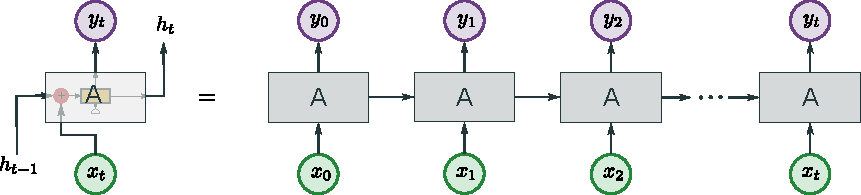
\includegraphics[width=1\textwidth]{images/Illustrationen/RNN_enrolled}
                    \caption{Darstellung einer \glqq ausgerollten\grqq \ und vereinfachten RNN Zelle}
                    \label{fig:RNN_enroled}
                \end{figure}
            Doch auch die RNNs haben ein Problem bei Merkmalen, die sich über einen längeren Zeitraum strecken.
            Denn dabei kommt es häufig vor, dass durch die Back Propagation die berechneten Gradienten entweder verschwindend klein, oder sehr groß werden.
            Gerade bei Abhängigkeiten über einen größeren zeitlichen Abstand tendieren die Fehlersignale,
            die durch die Back Propagation durch das Netz gegeben werden, zu geringe Gewichtsänderungen auszulösen.
            Traditionelle Aktivierungsfunktionen wie die hyperbolische Tangensfunktion haben Gradienten im Bereich $(-1,1)$ oder $[0,1)$ und Backpropagation berechnet Gradienten durch die Kettenregel.
            Dies hat den Effekt, dass n dieser kleinen Zahlen multipliziert werden, um die Gradienten der \glqq vorderen\grqq \ Schichten in einem n-Schichten-Netzwerk zu berechnen, was bedeutet, dass der Gradient (Fehlersignal) exponentiell mit n abnimmt und die vorderen Schichten sehr langsam trainieren.
            Die von Sepp Hochreiter erstmals erwähnte \textit{Long Short-Term Memory} (LSTM) Zellen ermöglichen durch verbesserte Fehlerkorrektur stabilere Lernergebnisse sowie auch das Lernen von Mustern mit noch größeren zeitlichen Abständen.~\cite{HOCHREITER1998}

            Diese Sonderform der RNNs, die auch in dieser Arbeit verwendet werden, sollen deshalb genauer untersucht werden.
            %% TODO Batch Normalisation \cite{LSTMbatchnorm}
   	
        \subsection{Long Short-Term Memory} 
            Hauptziel der LSTMs ist es, das Lernen der zeitlich abhängigen Muster zu verbessern.
            Entscheident dafür ist die Einschätzung welche zuvor gesehenen Informationen für die aktuelle Eingabe relevant sein könnten.
            
            \begin{figure}[h]
                \centering
                \includegraphics[width=0.8\textwidth]{images/Illustrationen/LSTM}
                \caption{Schematische Darstellung eines Knotens in einem LSTM NN, mit Input, Output und Forget Gate (inspiriert von \cite{OLAH2015}).}
                \label{fig:LSTM}
            \end{figure}

            Und um zu erlernen welche früheren Ausgaben für die Ermittlung nächster Datenpunkte entscheident sind, wird an jedem Knoten eine \textit{Memory Cell} \marginpar{zu dt. Gedächtniszelle} angebracht, zu sehen ist diese Erweiterung in Abbildung~\ref{fig:LSTM}.
            Sie ist mit sich selbst verbunden, kennt also die vorherigen Ausgaben und gibt den Zellstatus an.
            Mit Hilfe dieser Information soll eine Abhängigkeit auch über einen längeren Zeitraum gefunden werden.
            Der Zellstatus $C_{t-1}$ zum Zeitpunkt $t-1$ hat im nächsten Zeitschritt $t$ einen Einfluss auf den Zellstatus $C_{t}$ und somit auch auf die Ausgabe $y_t$.
            Die Weitergabe des Status wird in Abbildung~\ref{fig:LSTM_Status} dargestellt.

                \begin{figure}[h]
                    \centering
                    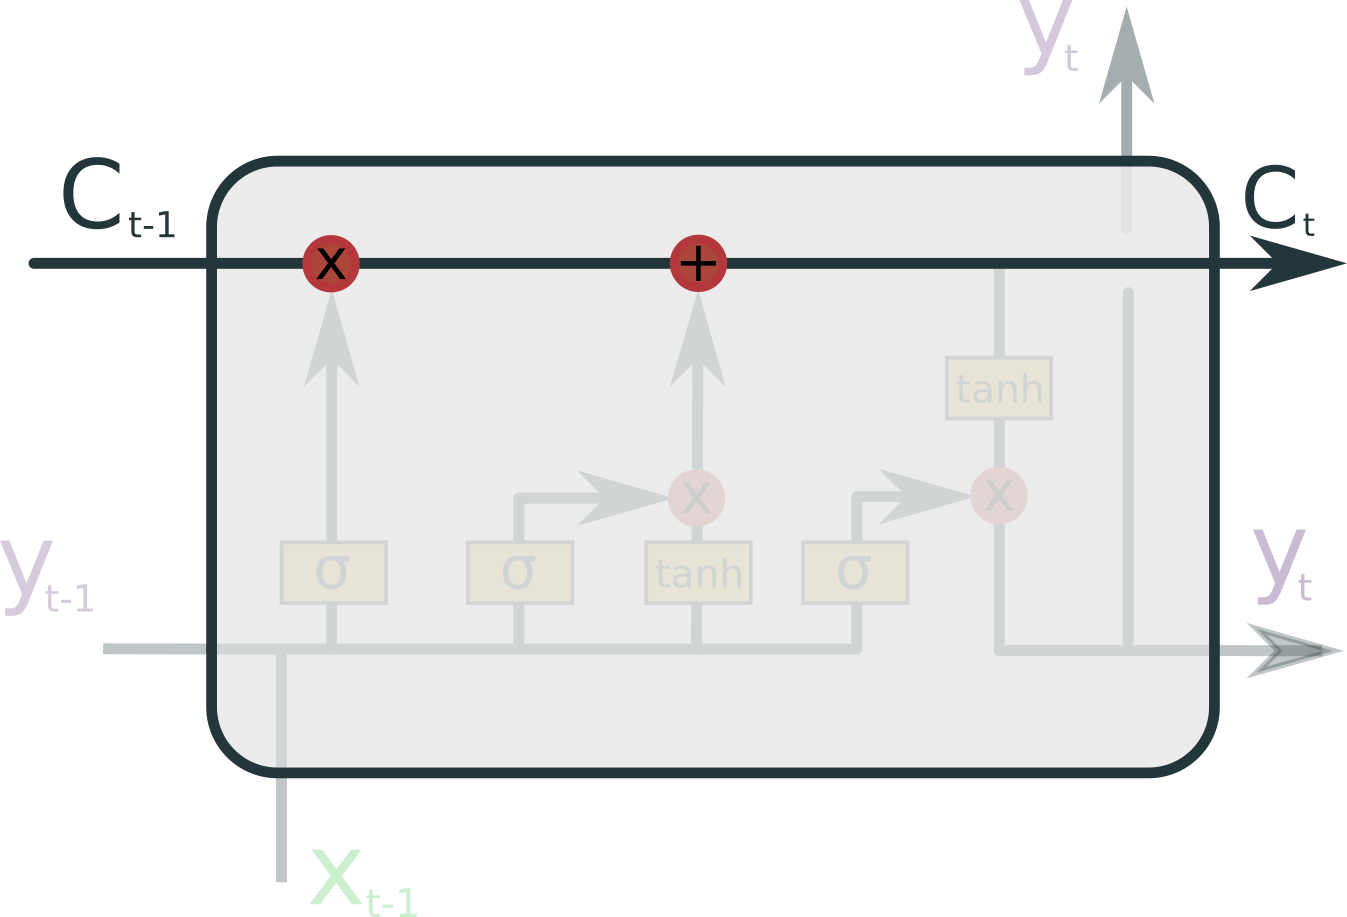
\includegraphics[width=0.5\textwidth]{images/Illustrationen/LSTM_MC}
                    \caption{Weitergabe des Zellstatus innerhalb eines Knotens (inspiriert von \cite{OLAH2015}).}
                    \label{fig:LSTM_Status}
                \end{figure}
                
                Einfluss auf den Zellstatus haben zwei verschiedene \textit{Gates} \marginpar{zu dt. Gatter/Tore}.
            Im ersten Schritt wird entschieden, welche Information aus dem vorherigen Zeitschritt keinen Einfluss mehr auf den Zellstatus haben sollen.
            Dies wird mit dem \textit{Forget Gate} umgesetzt und ist in Abbildung~\ref{fig:LSTM_Forget} zu sehen und kann analog zur RNN Zelle folgendermaßen hergeleitet werden.

            \begin{equation}
                f_t = \sigma\left(W_{fh}h_{t-1} + W_{fx}x_t + b_f\right)
            \end{equation}

            $W_{fh}$ und $W_{fx}$ beschreiben die Gewichte $b_f$ den Bias des \textit{Forget Gate}.
            Es wird also die vorherige Eingabe $h_{t-1}$ sowie die aktuelle Eingabe $x_t$ gewichtet und mit Bias an die Aktivierungsfunktion $\sigma$ übergeben.
            Damit sollen Informationen aus dem Speicher, die keinen Einfluss mehr haben sollen, entfernt werden.
            In dem Sprachbeispiel könnte das Genus (\textit{grammatikalisches Geschlecht}) gespeichert werden, um so eine grammatikalisch korrekte Vorhersage zu machen.
            Kommt nun allerdings ein neues Pronomen in der Eingabe $x_t$, sollte das bisher gespeicherte Genus keinen Einfluss mehr haben.
            
                \begin{figure}[h]
                    \centering
                    \includegraphics[width=0.5\textwidth]{images/Illustrationen/LSTM_FG}
                    \caption{Einfluss des Forget Gates auf den Zellstatus (inspiriert von \cite{OLAH2015}).}
                    \label{fig:LSTM_Forget}
                \end{figure}
                
            Das \textit{Input Gate} soll im nächsten Schritt angeben, welche neuen Informationen in den Zellstatus $C_t$ aufgenommen werden.
            Dies erfolgt in zwei Schritten, zunächst wird mit $i_t$ ermittelt, welche Information geupdated werden soll.

            \begin{equation}
                \begin{split}
                    i_t &= \sigma\left(W_{ih}h_{t-1} + W_{ix}x_t + b_i\right), \\
                    \tilde{C}_t &= tanh\left(W_{\tilde{C}h}h_{t-1} + W_{\tilde{C}x}x_t + b_{\tilde{C}}\right),\\
                \end{split}
            \end{equation}

            Im Vektor $\tilde{C}$ sind mögliche Kandidaten enthalten (wie z.B. das Genus), welcher den zuvor vergessenen Wert ersetzen soll (vgl. Abbildung~\ref{fig:LSTM_Input}).
            Der gesamte Zellstatus $C_t$ wird dann zusammen mit Werten aus dem \textit{Forget Get} verrechnet.

            \begin{equation}
                \begin{split}
                    C_t &=f_t\times C_{t-1} + i_t\times \tilde{C}_t, \\
                \end{split}
            \end{equation}

                \begin{figure}[h]
                    \centering
                    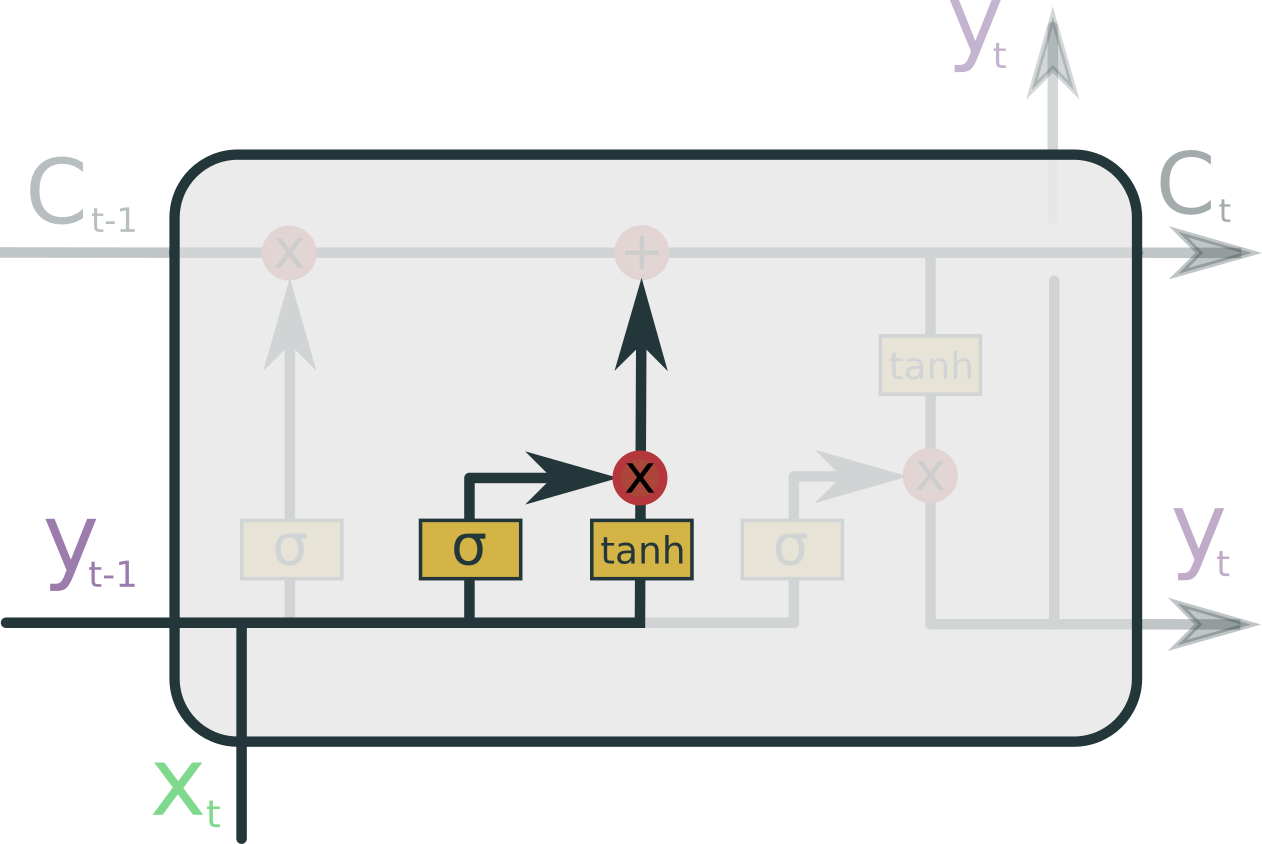
\includegraphics[width=0.5\textwidth]{images/Illustrationen/LSTM_IG}
                    \caption{Einfluss des Input Gates auf den Zellstatus (inspiriert von \cite{OLAH2015}).}
                    \label{fig:LSTM_Input}
                \end{figure}
            
            Wie der Zellstatus $C_t$ nun die Ausgabe beeinflusst, wird über das \textit{Output Gate} geregelt (siehe Abbildung~\ref{fig:LSTM_Output}).
            \begin{equation}
                \begin{split}
                    o_t &= \sigma\left(W_{oh}h_{t-1} + W_{ox}x_t + b_o \right), \\
                    h_t &= o_ttanh\left(c_t\right)
                \end{split}
            \end{equation}
            Dies soll in unserem Sprachbeispiel entscheiden, ob die Information des Genus für die Vorhersage des nächsten Wortes eine Rolle spielt. \cite{GERS2000} \cite{OLAH2015}

                \begin{figure}[h]
                    \centering
                    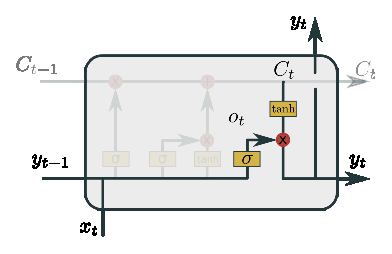
\includegraphics[width=0.5\textwidth]{images/Illustrationen/LSTM_OG}
                    \caption{Das Output Gate regelt den Einfluss des Zellstatus auf die Ausgabe des Neurons (inspiriert von \cite{OLAH2015}).}
                    \label{fig:LSTM_Output}
                \end{figure}
            
            Die verschiedenen Gates können so als ein weiteres kleines NN in jedem Knoten der LSTM Netze betrachtet werden, welche einen zeitlichen Zusammenhang besser erkennen sollen.
            Gesamt lässt sich eine LSTM Zelle mit den folgenden Formeln beschreiben:
            \begin{equation}
                \begin{split}
                    f_t &= \sigma\left(W_{fh}h_{t-1} + W_{fx}x_t + b_f\right) \\
                    i_t &= \sigma\left(W_{ih}h_{t-1} + W_{ix}x_t + b_i\right), \\
                    \tilde{C}_t &= tanh\left(W_{\tilde{C}h}h_{t-1} + W_{\tilde{C}x}x_t + b_{\tilde{C}}\right),\\
                    C_t &=f_t\times C_{t-1} + i_t\times \tilde{C}_t, \\
                    o_t &= \sigma\left(W_{oh}h_{t-1} + W_{ox}x_t + b_o \right), \\
                    h_t &= o_ttanh\left(c_t\right) \\
                    y_t &= h_t
                \end{split}
            \end{equation}
